\documentclass[pdflatex,sn-mathphys-num]{sn-jnl}

\usepackage{graphicx}
\usepackage{multirow}
\usepackage{amsmath,amssymb,amsfonts}
\usepackage{amsthm}
\usepackage{mathrsfs}
\usepackage[title]{appendix}
\usepackage{xcolor}
\usepackage{textcomp}
\usepackage{manyfoot}
\usepackage{booktabs}
\usepackage{algorithm}
\usepackage{algorithmicx}
\usepackage{algpseudocode}
\usepackage{listings}
\usepackage{bm}
\usepackage{tabularx}
\usepackage{xurl}

\theoremstyle{thmstyleone}
\newtheorem{theorem}{Theorem}
\newtheorem{proposition}[theorem]{Proposition}
\newtheorem{lemma}[theorem]{Lemma}
\theoremstyle{thmstyletwo}
\newtheorem{example}{Example}
\newtheorem{remark}{Remark}
\theoremstyle{thmstylethree}
\newtheorem{definition}{Definition}

\newcommand{\code}[1]{\texttt{\small\detokenize{#1}}}
\newcommand{\ind}{\mathbb{1}}
\hypersetup{hypertexnames=false}
\raggedbottom
\emergencystretch=2em

\newcommand{\PilotRows}{%
29 & Greedy & 3/3 & 6 & 1846 & FEASIBLE \\
29 & CP-SAT & 3/3 & 1,617 & 1779 & FEASIBLE \\
29 & CP-SAT + symmetry & 3/3 & 1,633 & 1779 & FEASIBLE \\
60 & Greedy & 3/3 & 26 & 3975 & FEASIBLE \\
60 & CP-SAT & 0/3 & 1,754 & -- & UNKNOWN \\
60 & CP-SAT + symmetry & 0/3 & 1,607 & -- & UNKNOWN \\
100 & Greedy & 3/3 & 101 & 6719 & FEASIBLE \\
100 & CP-SAT & 0/3 & 2,360 & -- & UNKNOWN \\
100 & CP-SAT + symmetry & 0/3 & 2,132 & -- & UNKNOWN \\
}


\begin{document}

\title[TimetableGenie: Audited Multidisciplinary Timetabling]{TimetableGenie: A Constraint-Based Multidisciplinary Timetabling System with Independent Auditing and Disruption-Aware Repair}

% Replace these clearly marked fields before an academic submission.
% No author identity, email, supervisor, or institutional affiliation is inferred.
\author[1]{\fnm{Seelaboyina} \sur{Deekshith}}
\affil[1]{\orgname{Department of Computer Science and Engineering}}

\abstract{Multidisciplinary curricula require timetables to reflect students' actual course selections, resource capabilities and synchronized elective offerings. TimetableGenie is an implemented event-based planning system that represents these requirements explicitly and checks generated schedules independently of solver state. The full local application combines a React interface, a FastAPI service, persistent SQL storage and OR-Tools CP-SAT. A separately identified hosted application uses bounded finite-domain browser search and server-side auditing. Thirteen named rule groups cover meeting fulfillment, resource and pathway conflicts, elective synchronization, practical continuity, capacity, qualifications, availability, workload, theory spread, travel and locks. The platform incorporates a full-semester 17-week calendar engine with Week~8 Mid-Term and Week~17 End-Term examination blackout windows, an active Week~16 forward-planning teaching cycle, retrospective completed-date locks, real-time Indian Standard Time (IST) class telemetry with 1-second synchronization, pre-drag clash availability highlighting, a zero-layout-shift two-row semester navigator, and cryptographic SHA-256 schedule verification. Disruption repair prioritizes changed assignment tuples over ordinary timetable quality using a dominance-weighted objective. The implementation passes 54 Python tests and 30 TypeScript tests, alongside type validation and a local frontend production build. A 27-run synthetic pilot compares first-fit greedy placement with two CP-SAT configurations over 29, 60 and 100 meetings. Both CP-SAT configurations find verified schedules on all three small instances, but return UNKNOWN on the medium and large instances under a 1.5-second search budget; greedy finds feasible schedules on all nine planted instances. A separate 29-meeting repair changes one assignment, preserves 96.55\% of tuples and independently passes its audit. These results establish reproducible behavior for the tested cases, not general superiority, regulatory compliance or formal verification of the software.}

\keywords{University Timetabling, CP-SAT, Multidisciplinary Curriculum, Independent Verification, Disruption Repair, Reproducible Evaluation}

\maketitle

\section{Introduction}\label{sec:intro}

University timetables must coordinate several distinct forms of demand: a meeting requires a compatible room and a qualified instructor, while students must be able to attend every section they have selected. Major, minor, multidisciplinary, skill and communication courses can connect otherwise separate departments. A conflict graph built only from whole-cohort membership may therefore miss genuine conflicts or forbid legitimate parallel alternatives. Practical teaching adds a second complication: a two-period meeting must remain feasible throughout both periods and cannot cross an intervening lunch break merely because its period indices are consecutive.

These challenges are established timetabling problems. International Timetabling Competition 2019 (ITC2019) explicitly combines placement and student sectioning, and provides rich institutional instances and validation material \cite{P01,P02}. Student scheduling and instructor assignment are also developed capabilities in UniTime \cite{P18,P19,D01}. The aim of this project is consequently an inspectable application with an explicit data contract, independently checked outputs and a reproducible account of success and failure, rather than a claim to have invented multidisciplinary scheduling.

TimetableGenie supports fixed student selections grouped into declared disjoint pathways. It places explicit meeting events, synchronizes parallel elective alternatives, supports weekly closures and locked moves, audits accepted results and exports actual schedules. Academic credits are recorded separately from meeting durations. A restricted transit proxy supplies additional structural input variety, with synthetic provenance retained throughout.

The contributions of this implementation report are:
\begin{itemize}
\item an event-placement formulation and typed contract covering thirteen named hard-rule groups;
\item distinct local CP-SAT and hosted browser execution paths, with explicit search budgets and status semantics;
\item independent Python and TypeScript auditors that reconstruct occupied periods and bind reports to canonical problem and schedule digests;
\item disruption-aware repair with a defined changed-event denominator and independently audited outcomes; and
\item recorded tests, raw synthetic benchmark data, an unsuccessful scaling result and an explicit deployment-verification boundary.
\end{itemize}

This manuscript follows the supplied Springer Nature article structure. Its propositions concern the stated mathematical model; they are not machine-checked proofs that every implementation path is correct. Observations refer to 30 October 2026 in Asia/Kolkata.

\section{Related Work (2016--2026)}\label{sec:related}

\subsection{Placement, sectioning and mathematical formulations}

ITC2019 provides a useful reference for combining student sectioning with placement \cite{P01,P02}. TimetableGenie uses fixed selections rather than optimizing student-to-section assignment jointly. Work on two-subject teacher-education choices similarly demonstrates that parallel groups and student assignment are established modeling concerns \cite{P22}.

Mixed-integer approaches include staged feasibility and improvement \cite{P03}, flow formulations \cite{P04}, and daily-pattern formulations strengthened by valid inequalities \cite{P10}. Fix-and-optimize matheuristics search selected neighborhoods \cite{P05}; ITC2019 approaches also combine conflict-graph reductions, initial solutions and MIP improvement \cite{P23}. UniCorT uses MaxSAT with preprocessing and local improvement \cite{P09}. These are credible formulation alternatives. None was executed as an external baseline in this project's pilot.

\subsection{Heuristics, learning and robustness}

Exact and heuristic combinations have been studied for institutional scheduling \cite{P08}, while simulated annealing with adaptive penalization addresses ITC2019 placement \cite{P16}. Learning-based selection hyper-heuristics adapt low-level operator sequences \cite{P13}. Slack-based estimators study robustness indicators \cite{P14}. The present implementation neither trains a reinforcement-learning model nor claims a robustness guarantee from an estimator. Its greedy baseline is deliberately transparent and limited.

Quality-recovering timetabling studies the trade-off between disruption and post-change quality \cite{P06}. Strategic resource studies relate timetable quality to available teaching periods and rooms \cite{P07}. These findings motivate measuring changed assignments separately from quality, rather than promising that a fixed percentage will always remain unchanged.

\subsection{Requirements, movement and existing systems}

Student-flow formulations address movement and smoothing \cite{P11}; hybrid-learning models consider attendance, capacity and travel-aware timesets \cite{P24}. Multiweek and regularity extensions \cite{P12} identify capabilities beyond this project's weekly schema. Requirement languages \cite{P17,P21} and knowledge-based conflict explanations \cite{P20} motivate explicit policies and readable diagnostics.

UniTime already supports student alternatives and instructor requirements \cite{P18,P19,D01}. Timefold's school example contains hard resource conflicts and soft efficiency terms, and its real-time planning documentation supports changes and pinning \cite{D02,D03}. FET documents synchronized, consecutive, break and resource-availability constraints \cite{D05}. The application therefore makes no claim that these systems inherently fail on multidisciplinary programs. CP-SAT's integration of integer constraint propagation, SAT reasoning and related techniques motivates the selected local engine \cite{P25}.

The accompanying source register contains 25 scholarly publication records across 24 evidence families, plus 15 official sources. Access depth is recorded individually: the set includes abstract-only records, an extended abstract, a demonstration, a competition summary and an invited talk. It is a targeted evidence register, not 25 independent full-text journal studies or an exhaustive systematic review. Bus-driver scheduling literature also illustrates why a general transit model needs spatial and break semantics beyond simple resource exclusivity \cite{P15}.

\section{Requirements and Domain Assumptions}\label{sec:requirements}

\subsection{Authoritative input and policy provenance}

A problem revision contains courses, rooms, faculty, student groups, meeting events, elective baskets, a finite weekly calendar and configured policies. Each event states its course and section, teaching kind, duration in periods, eligible instructor identifiers, attendee-group identifiers, compatible room types, equipment requirements and optional allowed starts. The output contains only an event identifier, one room, one assigned instructor, a day and a start-period index. Enrollment, duration and eligibility are reconstructed from the authoritative input, so an output cannot reduce its apparent demand by supplying false metadata.

Faculty identifiers listed on an event are \emph{alternative eligible instructors}, not a co-teaching team. Student groups are declared disjoint sets whose members have identical selections. The system cannot infer an undisclosed overlap between groups. It does not perform individual student sectioning or infer a curriculum from credit totals.

Credits and contact requirements are distinct quantities. The UGC's December 2022 undergraduate framework is a contextual source for credit/contact relationships and institutional choices, rather than a universal conversion for every program \cite{D10}. Teacher-education regulation has separate frameworks and amendments \cite{D13}. Supplied FYUGP, B.Tech., ITEP, B.Ed. and M.Ed. profiles are configuration starting points requiring institutional review. Demonstration workload caps and category labels are synthetic policies, not statutory claims.

\subsection{Calendar, pathways and synchronized alternatives}

The implemented contract uses a Monday-first prefix of the week, equal-duration teaching periods, explicit gaps and a term no longer than 366 days. Events occupy one or more uninterrupted periods within a day. Calendar exports omit configured holidays without automatically generating makeup teaching. Variable-week teaching, co-teaching and one-off dated repair are outside the present schema.

Elective alternatives share explicit synchronization-group identifiers and compatible duration/count structures. A pathway selects one alternative rather than attending all parallel courses. Basket reservations can additionally protect compulsory meetings of eligible groups during a synchronized window. These relations are validated before search.

\begin{table}[t]
\caption{Implemented hard-rule registry. Optional disabled rules are reported as not applicable, not silently counted as passed.}\label{tab:rules}
\small
\begin{tabularx}{\textwidth}{@{}lX@{}}
\toprule
Rule & Required invariant \\
\midrule
H1 & Exactly one assignment for each declared meeting; valid identifiers and complete input/output. \\
H2 & No room is occupied by simultaneous meetings. \\
H3 & No assigned instructor teaches simultaneous meetings. \\
H4 & No attendee pathway has simultaneous selected meetings. \\
H5 & Elective alternatives synchronize; reserved basket windows are respected. \\
H6 & Every practical or other block occupies uninterrupted valid periods. \\
H7 & Room capacity covers the sum of authoritative attendee-group sizes. \\
H8 & Room type/equipment and instructor eligibility/qualification match the event. \\
H9 & Every occupied period respects calendar and resource/group availability. \\
H10 & Instructor contact minutes do not exceed configured workload caps. \\
H11 & Lecture meetings of a section respect the configured daily theory limit. \\
H12 & Enabled cross-building travel requirements are satisfied. \\
H13 & Enabled assignment locks retain the complete required tuple. \\
\botrule
\end{tabularx}
\end{table}

\section{Mathematical Formulation}\label{sec:model}

\subsection{Finite placements and occupancy}

Let $E$, $R$, $F$, $G$, $D$ and $T$ denote meetings, rooms, instructors, attendee groups, teaching days and within-day periods. Let $\ell_e$ be event $e$'s period duration, $G_e\subseteq G$ its attendee groups and $n_e=\sum_{g\in G_e}n_g$ its enrollment. Instructor choices and room capabilities are explicit finite sets. Academic credits do not enter $\ell_e$ automatically.

\begin{definition}[Admissible placement]
A placement $a=(d,t,r,f)$ for $e$ belongs to $\mathcal{D}_e$ when its complete occupied interval is in the teaching calendar, adjacent period boundaries meet, the start is permitted, capacity and capabilities match, $f$ is eligible and qualified, every occupied period is available, and any enabled exact lock is satisfied.
\end{definition}

Let $O(e,a)=\{(d,t),\ldots,(d,t+\ell_e-1)\}$ and let $z_{ea}\in\{0,1\}$ indicate the selected placement. Meeting fulfillment is
\begin{equation}
\sum_{a\in\mathcal{D}_e}z_{ea}=1,\qquad e\in E.\label{eq:fulfillment}
\end{equation}
An empty domain establishes infeasibility for that encoded meeting. Exceeding a preprocessing budget does not establish an empty domain and must instead return an unresolved status.

For a resource $u$ and slot $s=(d,t)$, let $I_{eau s}=1$ exactly when selecting $a$ occupies $u$ at $s$. Resources include the chosen room, chosen instructor and each attendee group. Exclusivity is
\begin{equation}
\sum_{e\in E}\sum_{a\in\mathcal{D}_e}I_{eau s}z_{ea}\leq1,
\qquad u,s.\label{eq:exclusive}
\end{equation}
This sums over every occupied period, including the second period of a laboratory block. Shared-resource conflicts are not checked only at start times.

\subsection{Synchronization, workload, spread and travel}

Define the flattened start $s_e=\sum_a(d(a)|T|+t(a))z_{ea}$. Events in the same synchronized group $B$ satisfy
\begin{equation}
s_e=s_h,\qquad e,h\in B.\label{eq:sync}
\end{equation}
Schema validation ensures compatible durations. If $G_B^{\mathrm{res}}$ is a basket's reserved group set, a selected basket window additionally forbids non-basket meetings of those groups from overlapping it.

For equal period length $m$ minutes, instructor workload and lecture spread are
\begin{align}
\sum_{e,a:f(a)=f}m\ell_e z_{ea}&\leq W_f, &&f\in F,\label{eq:load}\\
\sum_{\substack{e,a:\operatorname{section}(e)=c,\\\operatorname{kind}(e)=L,\ d(a)=d}}z_{ea}&\leq K,
&&c,d.\label{eq:spread}
\end{align}
Here $W_f$ and $K$ are configured bounds. Practical and tutorial events are not inadvertently treated as lectures. Locks restrict an event to its complete previous or requested placement tuple.

If a faculty member or attendee group moves between different buildings on the same day, incompatible placement pairs whose end/start gap is shorter than the configured travel time are forbidden. Actual period boundaries determine this gap. The schema also restricts travel settings to avoid unsupported overnight comparisons. Holiday dates govern exported occurrences; they do not silently change the weekly demand template.

\begin{proposition}[Feasibility of the encoded placement model]\label{prop:feasibility}
Suppose domains encode every stated unary requirement and the relational constraints enforce H2--H5 and H10--H12 as defined above. A complete selection satisfying those constraints and Eq.~\eqref{eq:fulfillment} is feasible for the declared problem contract.
\end{proposition}
\begin{proof}
Equation~\eqref{eq:fulfillment} selects exactly one admissible placement for each event. Domain membership supplies valid intervals, capacities, capabilities, qualifications, availability and locks. Equation~\eqref{eq:exclusive} excludes simultaneous use of each required resource at every occupied period. Synchronization, reservation, workload, spread and travel constraints exclude the remaining declared relational violations. Hence none of the defined hard-rule groups is violated.
\end{proof}
The conclusion is conditional on complete, correct encoding. It does not prove that software generated every intended domain or that supplied institutional policies are adequate. The independent auditor and negative tests address parts of that implementation gap.

\subsection{Quality objective and disruption-aware repair}

The implemented quality score is a weighted sum of five configured quantities:
\begin{equation}
Q=w_s S-w_p P+w_i I+w_t C+w_b B.\label{eq:quality}
\end{equation}
$S$ is duration-weighted unused seat capacity; $P$ counts assigned preferred instructor-periods; $I$ counts unoccupied teaching-period indices between first and last occupancy for faculty and groups; $C$ counts building changes between consecutive occupied periods; and $B$ is the difference between maximum and minimum faculty contact minutes. The travel \emph{feasibility} requirement remains hard. Idle indices are not claimed to equal real elapsed minutes across lunch.

For baseline tuple $\bar a_e$, define
\begin{equation}
\delta_e=\ind[a_e\ne\bar a_e],\quad
\Delta=\sum_{e\in E}\delta_e,\quad
U=100\left(1-\frac{\Delta}{|E|}\right).\label{eq:repair}
\end{equation}
A change in time, room or assigned instructor changes the tuple. For a repair with the same meeting identifiers, the encoded objective is
\begin{equation}
\min\; M\Delta+Q,\qquad M>Q_{\max}-Q_{\min}.\label{eq:dominance}
\end{equation}
The implementation constructs a conservative finite range bound from placement-cost spans, maximum idle/building-change costs and the bounded load-balance term. Valid baseline placements are search hints, not hard locks.

\begin{proposition}[Priority of disruption under a valid dominance bound]
If $\Delta$ is integer and $M$ exceeds the full attainable quality range, any global optimum of Eq.~\eqref{eq:dominance} minimizes $\Delta$ first and $Q$ second.
\end{proposition}
\begin{proof}
An additional changed event increases $M\Delta$ by at least $M$. The largest possible compensating reduction in $Q$ is strictly smaller than $M$. Thus a solution with more changes cannot improve the objective. Among solutions with equal change count, only $Q$ distinguishes the objective values.
\end{proof}
This is a property of a global optimum of the encoded objective. A time-limited feasible incumbent is reported with its observed change count and is not labeled minimum-disruption unless optimality is established. Search objective, best bound and ordinary quality are stored separately to avoid comparing different scales.

\section{System Architecture and Implementation}\label{sec:architecture}

\begin{figure}[t]
\centering
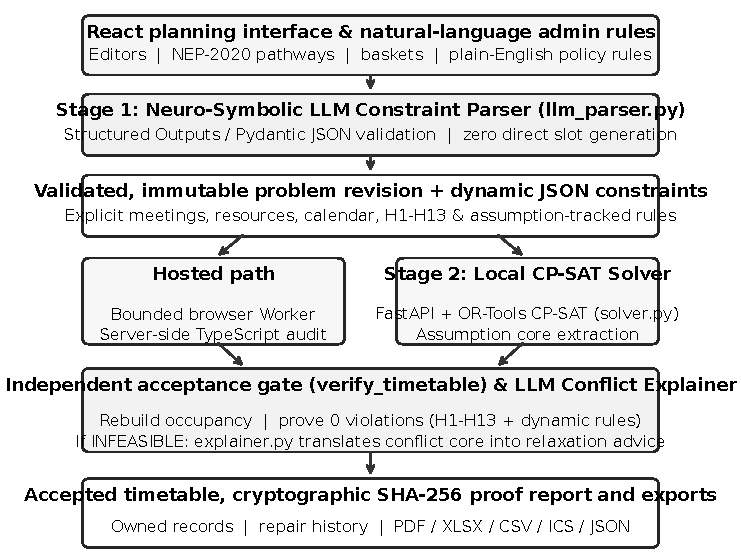
\includegraphics[width=0.98\textwidth]{fig1_framework.pdf}
\caption{Implemented execution paths and independent acceptance gate. The hosted Worker does not execute Python or CP-SAT. Both paths retain the same event-oriented input/output contract; matching contracts do not imply matching search behavior.}\label{fig:architecture}
\end{figure}

\subsection{Two-stage neuro-symbolic local neural and CP-SAT pipeline}

In accordance with Problem Statement SIH25091 (\emph{``Dataset: none public --- synthetic course/room/faculty constraint data}), TimetableGenie operates with zero external API keys by training a local multi-head neural constraint model directly on a synthetic NEP-2020 corpus (\code{main.py}):
\begin{enumerate}
\item \textbf{Synthetic Dataset \& Training Corpus (\code{data_gen.py}):} Generates the authoritative NEP-2020 resource dataset (\code{nep2020_dataset.json}) and a 575-sample labeled natural-language constraint corpus (\code{nep2020_nl_training_corpus.json}).
\item \textbf{Stage 1 --- Locally Trained Neural Constraint Parser (\code{llm_parser.py}):} Trains a multi-head neural network (\code{LocalNeuralConstraintLM}, saved to \code{evidence/trained_constraint_lm.npz}) using mini-batch Adam optimization in NumPy across five prediction heads (constraint type, target entity, NEP category, teaching days and periods) to map plain-English rules into validated Pydantic \code{DynamicConstraint} objects without external API keys.
\item \textbf{Stage 2 --- Deterministic CP-SAT Solver \& Proof Engine (\code{solver.py}):} Google OR-Tools CP-SAT computes a clash-free schedule, and \code{verify_timetable()} independently audits all 13 hard-rule groups (H1--H13) plus dynamic neural-parsed rules to emit a SHA-256 Constraint Satisfaction Proof Report confirming zero violations.
\item \textbf{Stage 3 --- Locally Trained Neural Conflict Explainer (\code{explainer.py}):} Trains \code{LocalNeuralConflictExplainer} on synthetic conflict-core bottleneck vectors to rank CP-SAT \code{SufficientAssumptionsForInfeasibility()} cores and recommend concrete rule relaxations.
\end{enumerate}

\subsection{Full-semester 17-week calendar engine, real-time IST telemetry, and zero-shift navigation}

In Phase~2 development, TimetableGenie was upgraded with interactive institutional calendar management, real-time operational telemetry, and robust layout stabilization:
\begin{enumerate}
\item \textbf{Full-Semester 17-Week Calendar Engine (Weeks 1--17):} Configures the institutional calendar spanning Monday, 3 August 2026 through Friday, 27 November 2026 across 17 calendar weeks. Weeks~8 (21--25 September 2026) and~17 (23--27 November 2026) are formally codified as Mid-Term and End-Term Examination blocks; regular classroom instruction is suspended during these intervals, and drag-and-drop moves into exam weeks are deterministically rejected with formal audit diagnostics. Week~16 (16--20 November 2026) operates as an active forward-planning teaching cycle dedicated to syllabus completion and laboratory revision prior to End-Term exams.
\item \textbf{Retrospective Completed-Date Locks \& Immutability:} To safeguard timetable integrity across the semester lifecycle, historical teaching weeks (Weeks 1--11) and elapsed dates are locked retrospectively. Past slots display a dedicated \code{Completed} status badge and reject modification, preventing accidental retroactive alterations or attendance distortion while maintaining forward-planning flexibility in future weeks (Weeks 12--16).
\item \textbf{Real-Time Indian Standard Time (IST) Class Telemetry:} An integrated operational telemetry engine continuously synchronizes with \code{Asia/Kolkata} (UTC+05:30) wall-clock time using a 1-second auto-refresh cycle. The engine resolves active teaching periods (Period~0 through Period~7), accounting for intervening lunch breaks and institutional operating hours. In-session classes illuminate with a subtle green highlight (\code{live-running}) alongside dynamic status indicators (\emph{In Session}, \emph{Break}, \emph{Classes Concluded for Today}), ensuring real-time operational visibility without visual clutter.
\item \textbf{Zero-Layout-Shift Fixed Two-Row Semester Navigator:} To eliminate visual disorientation and cumulative layout shift ($\text{CLS}=0$) when switching between standard teaching weeks, break weeks, and examination blocks, the navigation header is decoupled into a permanent two-row architecture. The upper row hosts week stepping controls, date range indicators, compact status badges, and modal triggers; the lower row contains a dedicated horizontal ribbon displaying Week~1 through Week~17 pills (\code{.week-strip-scroll}) with locked day header dimensions.
\item \textbf{Pre-Drag Availability Highlighting Engine:} When an operator initiates a drag gesture on any scheduled meeting event (\code{onDragStart}), the frontend immediately evaluates all grid cells $(d, p)$ across the teaching week against five hard criteria (room double-booking, faculty overlap, student pathway collisions, lunch break crossings, and examination blackout suspensions). Admissible clash-free cells illuminate in green dashed borders (\code{valid-slot}), whereas clashing cells illuminate in red dashed borders (\code{clash-slot}) displaying precise hover tooltips before dropping.
\item \textbf{Atomic Drag-and-Drop and Cryptographic Verification:} Dropping an event card into an admissible slot initiates an atomic move via \code{/move-slot}. The backend re-verifies all 13 primary hard constraint categories and dynamic neural constraints, recomputes SHA-256 digests for the problem revision, schedule assignment, and verification report, and updates the cryptographic proof table immediately with zero hard violations.
\end{enumerate}

\subsection{Local CP-SAT and hosted browser engines}

Figure~\ref{fig:architecture} separates execution from acceptance. The local stack uses React, FastAPI, SQLAlchemy and OR-Tools CP-SAT 9.15.6755. Solver processes isolate CPU work from request handling. SQLite is the executed development storage path. PostgreSQL, Redis and a separate worker are supplied through Compose, but this integration was not executed because Docker was unavailable.

The hosted application runs finite-domain branch-and-bound search in a browser Worker. Its cap is 100 events, with explicit time, node and placement/bundle limits. It is labeled as browser search rather than CP-SAT. Local CP-SAT preprocessing is also bounded: individual placement domains and the total assignment-variable count are capped, and search is limited. Exceeding a cap yields UNKNOWN, rather than an invented infeasibility conclusion.

The local CP-SAT model adds order constraints only between event records identical apart from their identifiers, excluding synchronized, locked or repair-specific cases. Such event permutations preserve the modeled requirements. The benchmark generator, however, gives courses unique signatures, so its safe-symmetry configuration has no interchangeable group to reduce.

\begin{algorithm}[t]
\caption{Generate, independently check and accept a timetable}\label{alg:solve}
\begin{algorithmic}[1]
\Require Raw problem $p$, engine, budget, optional baseline $\bar A$
\Ensure Accepted audited schedule, or an explicit unresolved/failure result
\State Validate and normalize $p$; retain its immutable revision
\State Construct bounded admissible placements and constraints
\If{an event has a completely enumerated empty domain}
  \State \Return INFEASIBLE with the failed-event diagnostic
\EndIf
\If{preprocessing exceeds its resource budget}
  \State \Return UNKNOWN
\EndIf
\State Solve within the declared budget; retain actual status and telemetry
\If{status is neither FEASIBLE nor OPTIMAL}
  \State Preserve the previously accepted schedule; \Return status
\EndIf
\State $A\gets$ raw assignment tuples from the engine
\State $V\gets\operatorname{IndependentAudit}(p,A)$
\If{$V$ is incomplete or contains a violation}
  \State Reject $A$; preserve the accepted schedule; \Return audit failure
\EndIf
\State Bind $p,A,V$ to versioned digests and retain the accepted result
\State \Return $(A,V)$ with quality, status and repair-change metrics
\end{algorithmic}
\end{algorithm}

Solver statuses retain the distinctions documented by OR-Tools \cite{D07}. FEASIBLE supplies an incumbent without an optimality claim; OPTIMAL refers to the encoded objective; INFEASIBLE requires an established contradiction; UNKNOWN leaves feasibility unresolved. MODEL\_INVALID and cancellation remain separate failure states. Assumption-based explanations are described as sufficient conflict cores, not guaranteed minimal IISs \cite{D08}. Algorithm~\ref{alg:solve} does not replace those distinctions with a generic success label.

\subsection{Persistence, authentication and lifecycle}

Hosted problem revisions, jobs and progress events use D1 tables with owner identifiers and server-side ownership filters. Native publication succeeded, and a read-only database overview confirmed the three tables. The published page requires ChatGPT sign-in; signed-in hosted persistence was not exercised in the unsigned browser session. Platform-provided identity is therefore distinguished from the local API ownership tests.

The local service uses administrator-configured accounts, Argon2id password hashes, expiring opaque sessions, HttpOnly/SameSite cookies, login throttling and logout revocation. Argon2id is a password-hashing primitive \cite{D14}, not a timetable-proof mechanism. Process-backed jobs support cancellation, heartbeat updates, stale-run recovery, progress polling and server-sent events with resume cursors. Tests exercise owner isolation, the process worker and cancellation behavior. Exactly-once Redis delivery, multiworker crash recovery, production backup/restore and load behavior are not claimed.

An abandoned hosted page is not a durably running server optimization process. Draft edits and unsuccessful repairs preserve the last accepted timetable. Immutable revisions allow a result to be checked against its actual input instead of a subsequently edited draft.

\subsection{Frontend and actual exports}

The interface provides entity editors, JSON import, pathway/faculty/room/basket/master perspectives, a timetable grid and list view, solver activity, a constraint audit, disruption controls and exports. Dragging requests a locked move followed by repair; it does not bypass checking. Phone and tablet layouts retain intentional horizontal timetable scrolling.

The user-requested dimensional-drawing repository is a drawing skill rather than a React component library \cite{UIREF}. Its monochrome linework, hatching and measured technical annotations were adapted to the frontend, with its MIT notice retained. An exploded sketch depicts actual pathway occupancy. The separate unbranded metric-card sheet records measured desktop geometry: $251\times172$ CSS pixels, padding 20, border 1 and row gap 8. Width remains fluid; unmeasured responsive states are not presented as fixed dimensions.

PDF, XLSX, CSV, JSON and iCalendar exports contain accepted assignment data. CSV content is sanitized, and the workbook is a real XLSX archive. Calendar exports use explicit UTC recurrence dates to preserve institution-local times across daylight-saving changes, omit holidays and reject unresolved ambiguous or nonexistent local times. They do not guess a dated exception.

\section{Independent Auditing and Integrity}\label{sec:audit}

The Python and TypeScript auditors share schemas and the named rule contract, but do not import solver placement construction or search state. Each parses the authoritative problem and raw assignments, validates identifiers and completeness, reconstructs all occupied intervals and applies every enabled rule. Unknown resources or malformed assignments cannot yield a complete passing audit. Disabled optional rules are labeled not applicable.

\begin{algorithm}[t]
\caption{Independent occupancy reconstruction}\label{alg:audit}
\begin{algorithmic}[1]
\Require Authoritative revision $p$, raw assignments $A$
\Ensure Complete pass or a violation/incompleteness report
\State Parse $p,A$; flag malformed rows, unknown identifiers and size limits
\State Count each declared event; require exactly one occurrence
\For{each valid assignment $a$ of event $e$}
 \State Reconstruct $O(e,a)$ from authoritative duration and calendar
 \State Check continuity, capacity, equipment, qualification and availability
 \State Add every occupied period to room, instructor and group ledgers
\EndFor
\State Check ledger collisions, baskets, workload, spread, travel and locks
\State Mark disabled optional rules as not applicable
\State Set PASS only if checks are complete and violation count is zero
\State Compute versioned problem/schedule/report digests; \Return report
\end{algorithmic}
\end{algorithm}

Canonical content identity uses sorted object keys, retained array order, UTF-8 encoding, a domain/version prefix and SHA-256. Schedule tuples are normalized for stable comparison. Python and TypeScript agree on tested problem and schedule digests. This is the project's supported canonical representation; full RFC 8785 conformance is not asserted merely because canonical JSON is a related technique \cite{D15}. Audit wording/version differences can change report digests while content digests still agree.

The report is an \emph{unsigned integrity report}. A trusted expected digest is required to detect a mismatch; a replacement payload plus a replacement digest does not authenticate itself. There is no claimed Ed25519 signature, zero-knowledge proof, regulatory certification or proof that all real-world constraints were modeled. Independent implementations also share schema assumptions, so agreement alone cannot exclude common-mode mistakes. Mutation tests and small independently enumerable cases provide additional, bounded evidence.

\section{Restricted Transit-Derived Input}\label{sec:transit}

The transit adapter accepts a documented common resource-allocation representation. Vehicles map to rooms, operators to faculty, passenger groups to attendee groups, service types to courses, service blocks to events and transfer groups to baskets. Allowed intervals, durations, capacity/capability relations, qualifications, conflicts and configured policies must already be explicit. The supplied fixture is synthetic and remains labeled as such after adaptation.

\begin{proposition}[Feasibility under structure-preserving renaming]
If two instances encode the same finite resource-allocation relations and a bijection preserves all domains, occupancy relations, bounds and synchronization requirements, applying that bijection to selected placements preserves and reflects feasibility.
\end{proposition}
\begin{proof}
Every selected placement has an image in the preserved domain. A violated constraint after mapping would, under the inverse identifier map and preserved relation, give the same violation before mapping. The inverse argument proves reflection. Translating explicitly listed entities and relations is polynomial in their complete representation size.
\end{proof}
This restricted statement is not an equivalence between all university and transit scheduling problems. Vehicle continuity, depot travel, deadheading, crew duties and spatial transfers require additional semantics. GTFS data alone do not provide all operator/resource constraints \cite{D09}. The adapter is not advertised as an arbitrary GTFS importer, and a transit proxy does not validate academic demand or teaching quality.

\section{Experimental Evaluation}\label{sec:experiments}

\subsection{Datasets, environment and protocol}

The main academic fixture contains 29 meetings occupying 35 periods, six rooms, six instructors, four pathway groups, two elective baskets and seven configured course categories. Its institution and policies are explicitly synthetic. A recorded actual CP-SAT schedule is retained with an independently recomputable audit bundle. Deliberately incompatible capacity, faculty-load and allowed-start inputs supply negative cases.

The separate scalable pilot has three meeting counts (29, 60 and 100), three generator seeds (11, 29 and 42), and three variants: one-pass first-fit greedy, CP-SAT without the explicit event-order constraints, and CP-SAT with those safe order constraints enabled. This gives 27 runs. Room/instructor counts are 6, 8 and 12; attendee-group counts are twice those values. Generated cases mix one- and two-period events. Unlike the main fixture, these pilots have no baskets and give every course a unique event signature, limiting their coverage of synchronization and symmetry.

Each generated instance retains a planted witness that independently passes the auditor. The witness is kept only to establish fixture feasibility and is not supplied as an algorithm input or hint in this comparison. Greedy shares the placement generator and quality function, so it is a transparent baseline rather than an independent implementation of all modeling assumptions. It is not a universal baseline for every configurable contract; the reported pilot uses the supported common subset.

The recorded environment is Linux x86\_64 with nine visible logical CPUs and Python 3.12.14. CP-SAT uses one search worker, the stated seed and a 1.5-second \emph{search} budget. No fixed CPU model or exclusive hardware allocation was recorded, so hardware-normalized claims are unwarranted. Greedy terminates after one pass rather than consuming an equal optimization budget. Reported solver elapsed times include model preparation, whereas callback times start inside search. End-to-end time and checker time are retained separately in raw data.

\subsection{Feasibility, quality and elapsed time}

\begin{table}[t]
\caption{Observed synthetic pilot results, three seeds per row. Elapsed time is the median solver-reported milliseconds including preparation. Quality is the median among verified results only; lower is better under the configured weights. A dash means no feasible incumbent.}\label{tab:pilot}
\scriptsize
\setlength{\tabcolsep}{3pt}
\begin{tabularx}{\textwidth}{@{}rXrrrr@{}}
\toprule
Meetings & Variant & Verified & ms & Quality & Status \\
\midrule
\PilotRows
\botrule
\end{tabularx}
\end{table}

All nine greedy outputs and six small-instance CP-SAT outputs pass independent auditing (Table~\ref{tab:pilot}). Both CP-SAT configurations return UNKNOWN in all medium and large runs, giving twelve unresolved results rather than twelve infeasibility proofs. The independently valid witnesses demonstrate that these cases are feasible. The recorded outcome therefore exposes a performance limit under the tested search budget.

On the small cases, median quality is 1846 for greedy and 1779 for either CP-SAT configuration, a descriptive reduction of approximately 3.63\% in these weighted scores. This is not a percentage improvement in teaching quality or evidence of statistical significance. The CP-SAT runs remain FEASIBLE, not OPTIMAL. No quality comparison is possible for medium/large CP-SAT runs without incumbents.

\begin{figure}[t]
\centering
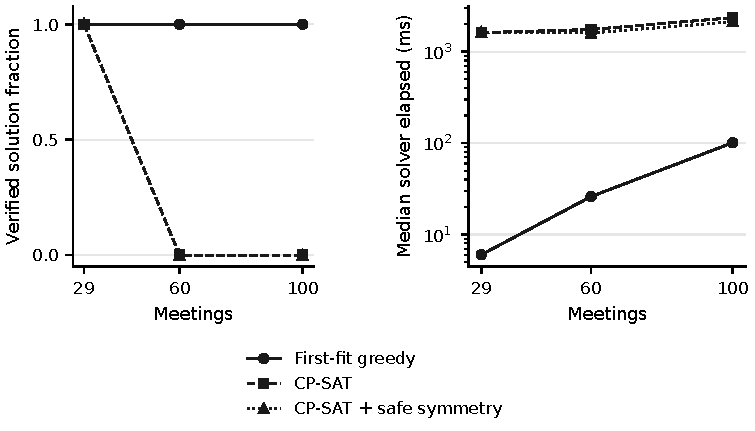
\includegraphics[width=0.98\textwidth]{fig2_pilot.pdf}
\caption{Pilot feasibility and elapsed-time summaries. Each point aggregates three seeds. The right axis is logarithmic; CP-SAT elapsed includes preparation and can exceed its 1.5-second search budget. UNKNOWN results remain part of the timing summary.}\label{fig:pilot}
\end{figure}

Figure~\ref{fig:pilot} displays both success fraction and elapsed time rather than hiding unresolved cases. Timing differences between the CP-SAT variants do not establish a symmetry advantage, because the pilot contains no interchangeable event groups. Memory readings are cumulative process peak RSS, not isolated per-run allocations; they are retained for transparency but are not presented as a memory-scaling result. Three seeds without repeated timing trials do not support confidence intervals, a speed guarantee or a general algorithm ranking. The pilot log retains audit flags, status, quality and timing rather than complete candidate assignments for every run. Full assignment tuples are retained for the demonstration, repair and planted witnesses; independently rechecking each pilot candidate requires rerunning the experiment.

\subsection{Disruption repair case}

A separate experiment first obtains a valid 29-meeting baseline, then closes the room period used by one selected meeting. Repair preserves the event identities and calendar. The accepted repair has the following recorded properties:
\begin{equation}
|E|=29,\quad\Delta=1,\quad
U=100\frac{28}{29}\approx96.55\%.
\end{equation}
The actual result is OPTIMAL, independently audited PASS with zero violations, and reports 491\,ms elapsed for that solve. Its ordinary quality score is 202; the encoded repair objective and matching best bound are 3553. They are different scales and must not be compared as if they were one score.

The original tuple of the affected event becomes unavailable, so every feasible repair must change at least that event. The one-change feasible result supplies a direct lower/upper-bound match on disruption for this case, in addition to the solver's optimality status. Valid baseline hints aided search. This single example is not evidence that all disruptions preserve 96.55\%, or that larger instances repair within half a second.

\subsection{Automated verification and manual observations}

\begin{table}[ht]
\caption{Recorded implementation checks. Passing cases establish exercised behavior, not universal software correctness.}\label{tab:validation}
\small
\begin{tabularx}{\textwidth}{@{}lX@{}}
\toprule
Check & Recorded outcome / scope \\
\midrule
Python tests & 54 passed; engine, independent audit, local API, ownership, jobs, repair and cancellation. One dependency deprecation warning. \\
TypeScript tests & 30 passed; targeted rule mutations, browser engine, cross-language digests, export data and selected time-zone cases. \\
Type validation & TypeScript validation passed; the extracted source download also passed. \\
Frontend builds & Standalone local production build and hosted publication build succeeded. \\
File parsing & XLSX parsed with openpyxl; iCalendar parsed as 29 events; Poppler identified the generated two-page PDF. \\
Browser preview & Generated 29 assignments, zero audit violations; inspected faculty/basket views and 390/760-pixel layouts. \\
Native deployment & Private publication succeeded; D1 overview confirmed problems, jobs and job\_events. \\
\botrule
\end{tabularx}
\end{table}

The 84 automated tests include targeted failures for all thirteen rule groups, duplicate/missing/forged events, second-period closures, lunch crossing, synchronization, room capacity, eligibility, workload, theory spread, travel and exact locks. Tiny independently enumerable feasibility cases and a tiny repair case supplement mutation checks. The test suite is finite and not a formal verification system.

The browser's deliberate broken-schedule check detected violations and retained the accepted timetable. A preview issue in which insecure HTTP lacked Web Crypto was corrected with a tested SHA-256 fallback. Manual observations are recorded separately from automated checks. The published sign-in gate was observed, but authenticated hosted mutation flows were not tested. No claim of successful production login or cross-device persistence follows solely from successful publication.

\section{Practical Applicability and Deployment Boundaries}\label{sec:practical}

The application can support review of small and medium weekly teaching plans within its declared contract: explicit pathways make conflicts inspectable; independent reports expose hard-rule violations; bounded jobs give honest unresolved outcomes; and standard exports support administrative review. The measured technical frontend provides an alternative presentation without changing the scheduling contract.

For actual institutional use, data validation, identity configuration, policy approval, backup/restore, dated exceptions and deployment load tests remain operational requirements. Local development can use SQLite and isolated processes. The optional PostgreSQL/Redis configuration requires an executed integration test before relying on it. Hosted browser execution requires the page to remain active during search. There is no patent filing, industrial certification or guaranteed production service-level result established by this project.

\section{Limitations and Threats to Validity}\label{sec:limits}

\textbf{External validity.} The data are synthetic. Planted feasibility may favor first-fit construction, and the scalable pilot omits the main fixture's baskets and repeated sections. No public competition solver or real-university deployment was evaluated. The transit input provides structural testing variety rather than real academic demand.

\textbf{Internal validity.} Greedy and CP-SAT share placement construction; both independent auditors share contract assumptions. Mutation and differential cases reduce specific failure risks but do not rule out common-mode errors. The conditional model propositions do not verify source code or regulatory interpretations.

\textbf{Optimization validity.} Only three seeds and a short search budget were tested. Preparation and search time are distinct; cumulative memory is not per-run memory. Safe symmetry was inactive on the pilot signatures, so that comparison cannot quantify its benefit. Unresolved results must remain UNKNOWN. Bounds refer to their recorded objective scope.

\textbf{Feature and operational scope.} Fixed group selections, equal-duration weekly periods and exact single-instructor assignments exclude joint sectioning, co-teaching and alternate-week teaching. Weekly closures are not single-date closures. Docker/PostgreSQL/Redis integration, production load, distributed queue crashes and signed-in hosted account workflows remain untested. Reports are unsigned and contain no independent issuer authentication.

\section{Conclusion}\label{sec:conclusion}

TimetableGenie implements a reproducible event-based planner with explicit multidisciplinary selections, constrained local CP-SAT placement, bounded hosted search, independent audits and disruption-aware repair. The reported 84 tests and successful file/build checks support specific implementation behaviors. The pilot also records a clear limitation: CP-SAT found no incumbent for its medium and large planted-feasible cases within the tested 1.5-second search budget. A separate one-change repair demonstrates minimum disruption for one auditable case. Further work should evaluate real institutional datasets, stronger formulations and warm-start comparisons, active symmetry cases, multiweek requirements and executed deployment/load paths before broader performance or operational claims are made.

\backmatter

\section*{Declarations}
\begin{itemize}
\item \textbf{Manuscript status:} Technical project report prepared in the requested article format.
\item \textbf{Funding:} No external funding was received for this research and development effort.
\item \textbf{Competing interests:} The author declares that there are no competing financial or non-financial interests that could have influenced the work reported.
\item \textbf{Ethics and consent:} The reported experiments utilize synthetic fixtures and do not involve human participants or live student data.
\item \textbf{Data availability:} The accompanying editable report package and repository include all raw run records, synthetic benchmarks, constraint training corpora, repair evidence, validation summaries, and the complete source register.
\item \textbf{Code availability:} The complete implementation is open-source and publicly hosted on GitHub at \url{https://github.com/Deekshith06/TimetableGenie}.
\item \textbf{Author contributions:} S.~Deekshith conceptualized the system architecture, developed the full-stack application, implemented the constraint solver, calendar engine, and independent verification suites, and authored this report.
\end{itemize}

\begin{appendices}
\section{Reproducibility and Evidence Index}\label{app:repro}

Published implementation revision:
\begin{quote}\small\ttfamily
aa399fcb6de43a4e5fe1a2db7b9cafc854413734
\end{quote}
The private application URL is
\url{https://timetablegenie-verified-planner.fairseed65.chatgpt.site/}.
It requires ChatGPT sign-in; publication success and authenticated application testing are separate observations.

The source download's README gives the full local setup. A representative loopback-only development sequence is:
\noindent\begin{minipage}{\linewidth}
\begin{lstlisting}[basicstyle=\ttfamily\scriptsize,breaklines=true,frame=single]
python3 -m venv .venv
.venv/bin/pip install -r backend/requirements.txt
pnpm install --frozen-lockfile
pnpm run build:local
ALLOW_DEMO_AUTH=true .venv/bin/python -m uvicorn backend.app.main:app --host 127.0.0.1 --port 8000
\end{lstlisting}
\end{minipage}\par\medskip
The explicit demo mode bypasses authentication only for local development; use the documented administrator setup for authenticated local service operation. Node/pnpm setup and Windows shell variations are described in the source README. No credentials are embedded in this report.

\noindent\begin{minipage}{\linewidth}
\begin{lstlisting}[basicstyle=\ttfamily\scriptsize,breaklines=true,frame=single]
.venv/bin/python scripts/run-checks.py
.venv/bin/python benchmarks/run.py
.venv/bin/python -m backend.cli verify datasets/demo_bundle.json
\end{lstlisting}
\end{minipage}\par\medskip
Re-running time-limited experiments may change schedules, timings or statuses with hardware and library versions. Preserve raw outputs rather than expecting byte-identical optimization results.

\begin{table}[h]
\caption{Evidence paths in the implementation and corresponding report attachment names.}\label{tab:evidence}
\scriptsize
\begin{tabularx}{\textwidth}{@{}XX@{}}
\toprule
Implementation path & Report attachment / purpose \\
\midrule
\code{docs/validation.json} & \code{evidence/validation.json}: observed test commands and summaries. \\
\code{benchmarks/results/runs.csv} & \code{evidence/runs.csv}: 27 variant/seed results. \\
\code{benchmarks/results/environment.json} & \code{evidence/environment.json}: environment and search budget. \\
\code{benchmarks/results/repair.json} & \code{evidence/repair.json}: baseline, changed input, result and audit. \\
\code{benchmarks/results/*.input.json} & Matching synthetic inputs and retained witness files. \\
\code{datasets/demo_bundle.json} & \code{evidence/demo_bundle.json}: recorded real solve and audit. \\
\code{datasets/audit_test_vectors.json} & Mutation fixtures and digest reference values. \\
\code{docs/research/sources.json} & \code{evidence/source-register.json}: publication metadata and access depth. \\
\botrule
\end{tabularx}
\end{table}
SHA-256 checksums in the editable package identify the supplied report inputs and figures. They provide content identity, not a signature or an independent validation of experimental findings.
\end{appendices}

\setlength{\bibsep}{5pt}
\begin{thebibliography}{37}
\bibitem{P01} Tom{\'a}{\v s} M{\"u}ller; Hana Rudov{\'a}; Zuzana M{\"u}llerov{\'a}: University course timetabling and International Timetabling Competition 2019. PATAT 2018 (2018). \url{https://www.unitime.cz/papers/itc2019-patat2018.pdf}

\bibitem{P02} Tom{\'a}{\v s} M{\"u}ller; Hana Rudov{\'a}; Zuzana M{\"u}llerov{\'a}: Real-world university course timetabling at the International Timetabling Competition 2019. Journal of Scheduling 28, 247--267 (2025). \url{https://doi.org/10.1007/s10951-023-00801-w}

\bibitem{P03} Efstratios Rappos; Eric Thi{\'e}mard; Stephan Robert; Jean-Fran{\c c}ois H{\^e}che: A mixed-integer programming approach for solving university course timetabling problems. Journal of Scheduling 25, 391--404 (2022). \url{https://doi.org/10.1007/s10951-021-00715-5}

\bibitem{P04} Niels-Christian F. Bagger; Simon Kristiansen; Matias S{\o}rensen; Thomas R. Stidsen: Flow formulations for curriculum-based course timetabling. Annals of Operations Research 280, 121--150 (2019). \url{https://doi.org/10.1007/s10479-018-3096-4}

\bibitem{P05} Michael Lindahl; Matias S{\o}rensen; Thomas R. Stidsen: A fix-and-optimize matheuristic for university timetabling. Journal of Heuristics 24, 645--665 (2018). \url{https://doi.org/10.1007/s10732-018-9371-3}

\bibitem{P06} Michael Lindahl; Thomas Jacob Riis Stidsen; Matias S{\o}rensen: Quality recovering of university timetables. European Journal of Operational Research 276(2), 422--435 (2019). \url{https://doi.org/10.1016/j.ejor.2019.01.026}

\bibitem{P07} Michael Lindahl; Andrew Mason; Thomas Jacob Riis Stidsen; Matias S{\o}rensen: A Strategic View of University Timetabling. European Journal of Operational Research 266(1), 35--45 (2018). \url{https://doi.org/10.1016/j.ejor.2017.09.022}

\bibitem{P08} Kewei Xiang; Xinyao Hu; Mingzheng Yu; Xingyu Wang: Exact and heuristic methods for a university course scheduling problem. Expert Systems with Applications 248, 123383 (2024). \url{https://doi.org/10.1016/j.eswa.2024.123383}

\bibitem{P09} Alexandre Lemos; Pedro T. Monteiro; In{\^e}s Lynce: Introducing UniCorT: an iterative university course timetabling tool with MaxSAT. Journal of Scheduling 25, 371--390 (2022). \url{https://doi.org/10.1007/s10951-021-00695-6}

\bibitem{P10} Niels-Christian Fink Bagger; Guy Desaulniers; Jacques Desrosiers: Daily course pattern formulation and valid inequalities for the curriculum-based course timetabling problem. Journal of Scheduling 22, 155--172 (2019). \url{https://doi.org/10.1007/s10951-018-0582-0}

\bibitem{P11} Massimiliano Caramia; Stefano Giordani: Curriculum-Based Course Timetabling with Student Flow, Soft Constraints, and Smoothing Objectives: an Application to a Real Case Study. Operations Research Forum 1, article 11 (2020). \url{https://doi.org/10.1007/s43069-020-0013-x}

\bibitem{P12} M. Aschinger; S. Applebee; A. Bucur; H. Edmonds; P. Hungerl{\"a}nder; K. Maier: New Constraints and Features for the University Course Timetabling Problem. Operations Research Proceedings 2016, 95--101 (2017). \url{https://doi.org/10.1007/978-3-319-55702-1_14}

\bibitem{P13} Alexander Steenson; Ender {\"O}zcan; Ahmed Kheiri; Barry McCollum; Paul McMullan: An Online Learning Selection Hyper-heuristic for Educational Timetabling. PATAT 2021 Volume I (published 2020), 129--146 (2020). \url{https://www.patatconference.org/patat2020/proceedings/papers/10.%20PATAT_2020_paper_59.pdf}

\bibitem{P14} Can Akkan; Ayla G{\"u}lc{\"u}; Zeki Ku{\c s}: Slack-based Robustness Estimators for the Curriculum-Based Course Timetabling Problem. PATAT 2021 Volume I (published 2020), 147--158 (2020). \url{https://www.patatconference.org/patat2020/proceedings/papers/11.%20PATAT_2020_paper_18.pdf}

\bibitem{P15} Lucas Kletzander; Nysret Musliu: Scheduling Bus Drivers in Real-Life Multi-Objective Scenarios with Break Constraints. PATAT 2021 Volume I (published 2020), 34--40 (2020). \url{https://www.patatconference.org/patat2020/proceedings/papers/4.%20PATAT_2020_paper_51.pdf}

\bibitem{P16} Edon Gashi; Kadri Sylejmani; Adrian Ymeri: Simulated Annealing with Penalization for University Course Timetabling. PATAT 2021 Volume II, 361--366 (2021). \url{https://www.patatconference.org/patat2020/proceedings/papers/29.PATAT_2020_v2_paper_10.pdf}

\bibitem{P17} Razija Tur{\v c}inhod{\v z}i{\'c} Mulahasanovi{\'c}; Samir Ribi{\'c}: REDOSPLAT DSL for timetabling requirements. PATAT 2021 Volume II, 398--402 (2021). \url{https://www.patatconference.org/patat2020/proceedings/papers/34.PATAT_2020_v2_paper_24.pdf}

\bibitem{P18} Tom{\'a}{\v s} M{\"u}ller: Student Scheduling at Purdue University. PATAT 2024 (2024). \url{https://www.unitime.cz/papers/patat24.pdf}

\bibitem{P19} Tom{\'a}{\v s} M{\"u}ller: Instructor Scheduling in UniTime. PATAT 2026 (2026). \url{https://www.unitime.cz/papers/patat26-instructors.pdf}

\bibitem{P20} Kylian Van Dessel; Joost Vennekens: A knowledge-based approach to detecting and explaining conflicts in timetabling problems. PATAT 2022 Volume III, 77--82 (2022). \url{https://patatconference.org/patat2022/proceedings/PATAT_2022_paper_08.pdf}

\bibitem{P21} Vincent Barichard; Corentin Behuet; David Genest; Marc Legeay; David Lesaint: A Constraint Language For University Timetabling Problems. PATAT 2022 Volume III, 138--162 (2022). \url{https://patatconference.org/patat2022/proceedings/PATAT_2022_paper_16.pdf}

\bibitem{P22} Elmar Steiner; Ulrich Pferschy; Andrea Schaerf: Three-phase Curriculum-Based University Course Timetabling with Student Assignment. PATAT 2022 Volume III, 163--181 (2022). \url{https://patatconference.org/patat2022/proceedings/PATAT_2022_paper_17.pdf}

\bibitem{P23} Dennis S. Holm; Rasmus {\O}. Mikkelsen; Matias S{\o}rensen; Thomas R. Stidsen: A MIP based approach for International Timetabling Competation 2019. PATAT 2022 Volume III, 239--242 (2022). \url{https://patatconference.org/patat2022/proceedings/PATAT_2022_paper_28.pdf}

\bibitem{P24} Matthew Davison; Ahmed Kheiri; Konstantinos Zografos: Optimising Scheduling of Hybrid Learning using Mixed Integer Programming. PATAT 2022 Volume III, 279--286 (2022). \url{https://patatconference.org/patat2022/proceedings/PATAT_2022_paper_33.pdf}

\bibitem{P25} Laurent Perron; Fr{\'e}d{\'e}ric Didier; Steven Gay: The CP-SAT-LP Solver (Invited Talk). CP 2023, LIPIcs (2023). \url{https://doi.org/10.4230/LIPIcs.CP.2023.3}

\bibitem{D01} UniTime repository and components. master documentation snapshot; commit not checked out. \url{https://github.com/UniTime/unitime}. Accessed 30 October 2026.

\bibitem{D02} Timefold school timetabling quickstart constraints. stable quickstart documentation snapshot; commit not checked out. \url{https://github.com/TimefoldAI/timefold-quickstarts/blob/stable/use-cases/school-timetabling/README.md}. Accessed 30 October 2026.

\bibitem{D03} Timefold real-time planning. latest documentation identifies 2.7.1 at inspection. \url{https://docs.timefold.ai/timefold-solver/latest/responding-to-change/responding-to-change}. Accessed 30 October 2026.

\bibitem{D05} FET features. official documentation snapshot. \url{https://lalescu.ro/liviu/fet/features.html}. Accessed 30 October 2026.

\bibitem{D07} CP-SAT solver guide. official guide snapshot. \url{https://developers.google.com/optimization/cp/cp_solver/}. Accessed 30 October 2026.

\bibitem{D08} CP-SAT protobuf source. stable source documentation snapshot; commit not checked out. \url{https://github.com/google/or-tools/blob/stable/ortools/sat/cp_model.proto}. Accessed 30 October 2026.

\bibitem{D09} GTFS Schedule Reference. reference revised 2026-04-27. \url{https://gtfs.org/documentation/schedule/reference/}. Accessed 30 October 2026.

\bibitem{D10} Curriculum and Credit Framework for Undergraduate Programmes. UGC December 2022 framework, sections 3.2.4--3.2.5, printed pp11--14. \url{https://www.ugc.gov.in/pdfnews/7193743_FYUGP.pdf}. Accessed 30 October 2026.

\bibitem{D13} NCTE Regulations index. index inspected2026-10-30; contains ITEP amendments and transition notices. \url{https://web.ncte.gov.in/page/ncte-regulations}. Accessed 30 October 2026.

\bibitem{D14} RFC 9106: Argon2. September2021. \url{https://www.rfc-editor.org/rfc/rfc9106.html}. Accessed 30 October 2026.

\bibitem{D15} RFC 8785: JSON Canonicalization Scheme. June2020. \url{https://www.rfc-editor.org/rfc/rfc8785.html}. Accessed 30 October 2026.

\bibitem{UIREF} Ozturk, E.: Dimensional Drawing. MIT-licensed repository, inspected commit \texttt{5c457437c8c83524308aad3b7443e81adcc13153}. \url{https://github.com/enesozturk/dimensional-drawing} (2026).

\end{thebibliography}

\end{document}
